% Written by make_prompt_figures.py (question 3159). The images are 17 cm wide, a single-column A4 text block with 2 cm margins.
\begin{figure}[t]
\centering
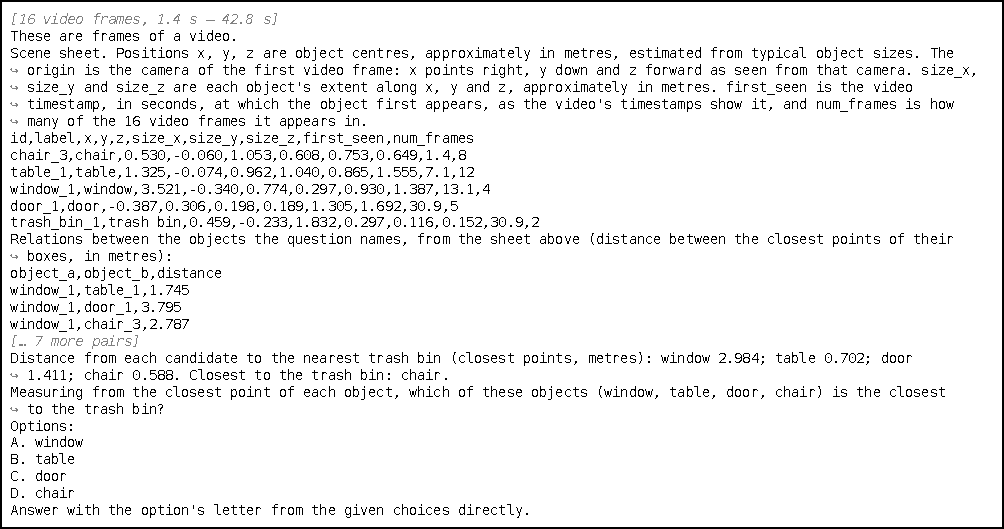
\includegraphics[width=\linewidth]{figures/prompt_example_pipeline_v4.pdf}
\caption{The text Qwen3.5-2B receives after the video for one VSI-Bench question (3159, relative distance) with the pipeline\_v4 scene sheet. Each sheet row is one tracked object: \texttt{id} and \texttt{label}; \texttt{x, y, z}, its centre, and \texttt{size\_x, size\_y, size\_z}, its extent, in the coordinates of the first frame's camera (x right, y down, z forward), scaled to approximately metres from typical object sizes; \texttt{first\_seen}, the video timestamp at which it first appears; \texttt{num\_frames}, in how many of the 16 frames it is seen. For distance questions the sheet keeps one row per object the question names, then lists the closest-point distances between their boxes, and a relation line states each candidate's distance to the reference object and which is closest. Grey text is not part of the prompt; left out: 7 of the 10 distance pairs.}
\label{fig:prompt-pipeline-v4}
\end{figure}

\begin{figure}[t]
\centering
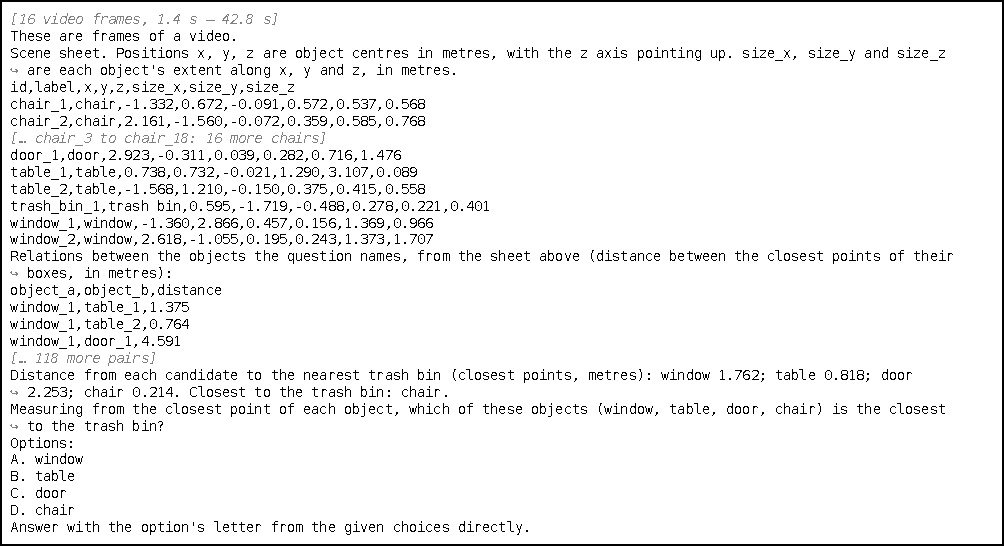
\includegraphics[width=\linewidth]{figures/prompt_example_gold.pdf}
\caption{The same question (3159) with the gold scene sheet and its relations (condition C): VSI-Bench's labelled objects instead of the pipeline's. \texttt{x, y, z} are box centres and \texttt{size\_x, size\_y, size\_z} box extents, in metres in the dataset's world frame (z up); gold sheets have no timestamps. The relation table gives the closest-point distance between every two objects of the named classes, and the relation line each candidate's distance to the nearest reference object. Grey text is not part of the prompt; left out: 16 of the 24 sheet rows, 118 of the 121 distance pairs.}
\label{fig:prompt-gold}
\end{figure}
